
\chapter{Discussion}
\label{ch:discussion}

\section{The number that gets reported and the number that matters}

Published accuracies above 99\,\% on PlantVillage are not wrong. They are answers to
the question the dataset asks. The problem is that the answer is easy to quote out of
context, and once quoted it displaces the harder question.

Our measurement puts the two side by side on the same checkpoints: 0.9931 macro-F1 on
held-out curated images, 0.1798 on field images. The gap is 81 points, which is
large enough that the two numbers describe different systems rather than different
measurements of one system.

\section{Why the shortcut explanation was wrong in its strong form}

The tempting account of the gap is that the model learned to read the background.
Soil, hands, pots and laboratory surfaces correlate with disease category in curated
data because collection was organised by category, so a network can fit the label
from context alone.

The swap test says something more specific. Background content can move the
prediction 21.8\,\% of the time, which is far above chance and means the shortcut is
real. But leaf content moves it 50.3\,\% of the time, more than twice as often. The
model is not ignoring the plant.

This distinction matters for what to do next. If the model were reading background
instead of leaf, fixing the background would fix the model. It does not, and the
augmentation experiment confirms that it does not.

\section{Why the fix failed, and why that was predictable}

Background augmentation buys invariance to a factor the model is not primarily using
for identity. It therefore cannot repair a gap caused by the factor the model is
using, which is leaf appearance.

The prediction recorded before the run was that augmentation would recover a portion
of the gap and not most of it. The measured effect is 1.6\,\% of the gap, with an
interval spanning zero. Direction and magnitude agree, and the agreement is worth
more than the number, because it means the mechanism measurement has predictive
force rather than being a post-hoc story.

\section{What the failure modes look like}

\begin{figure}[H]
\centering
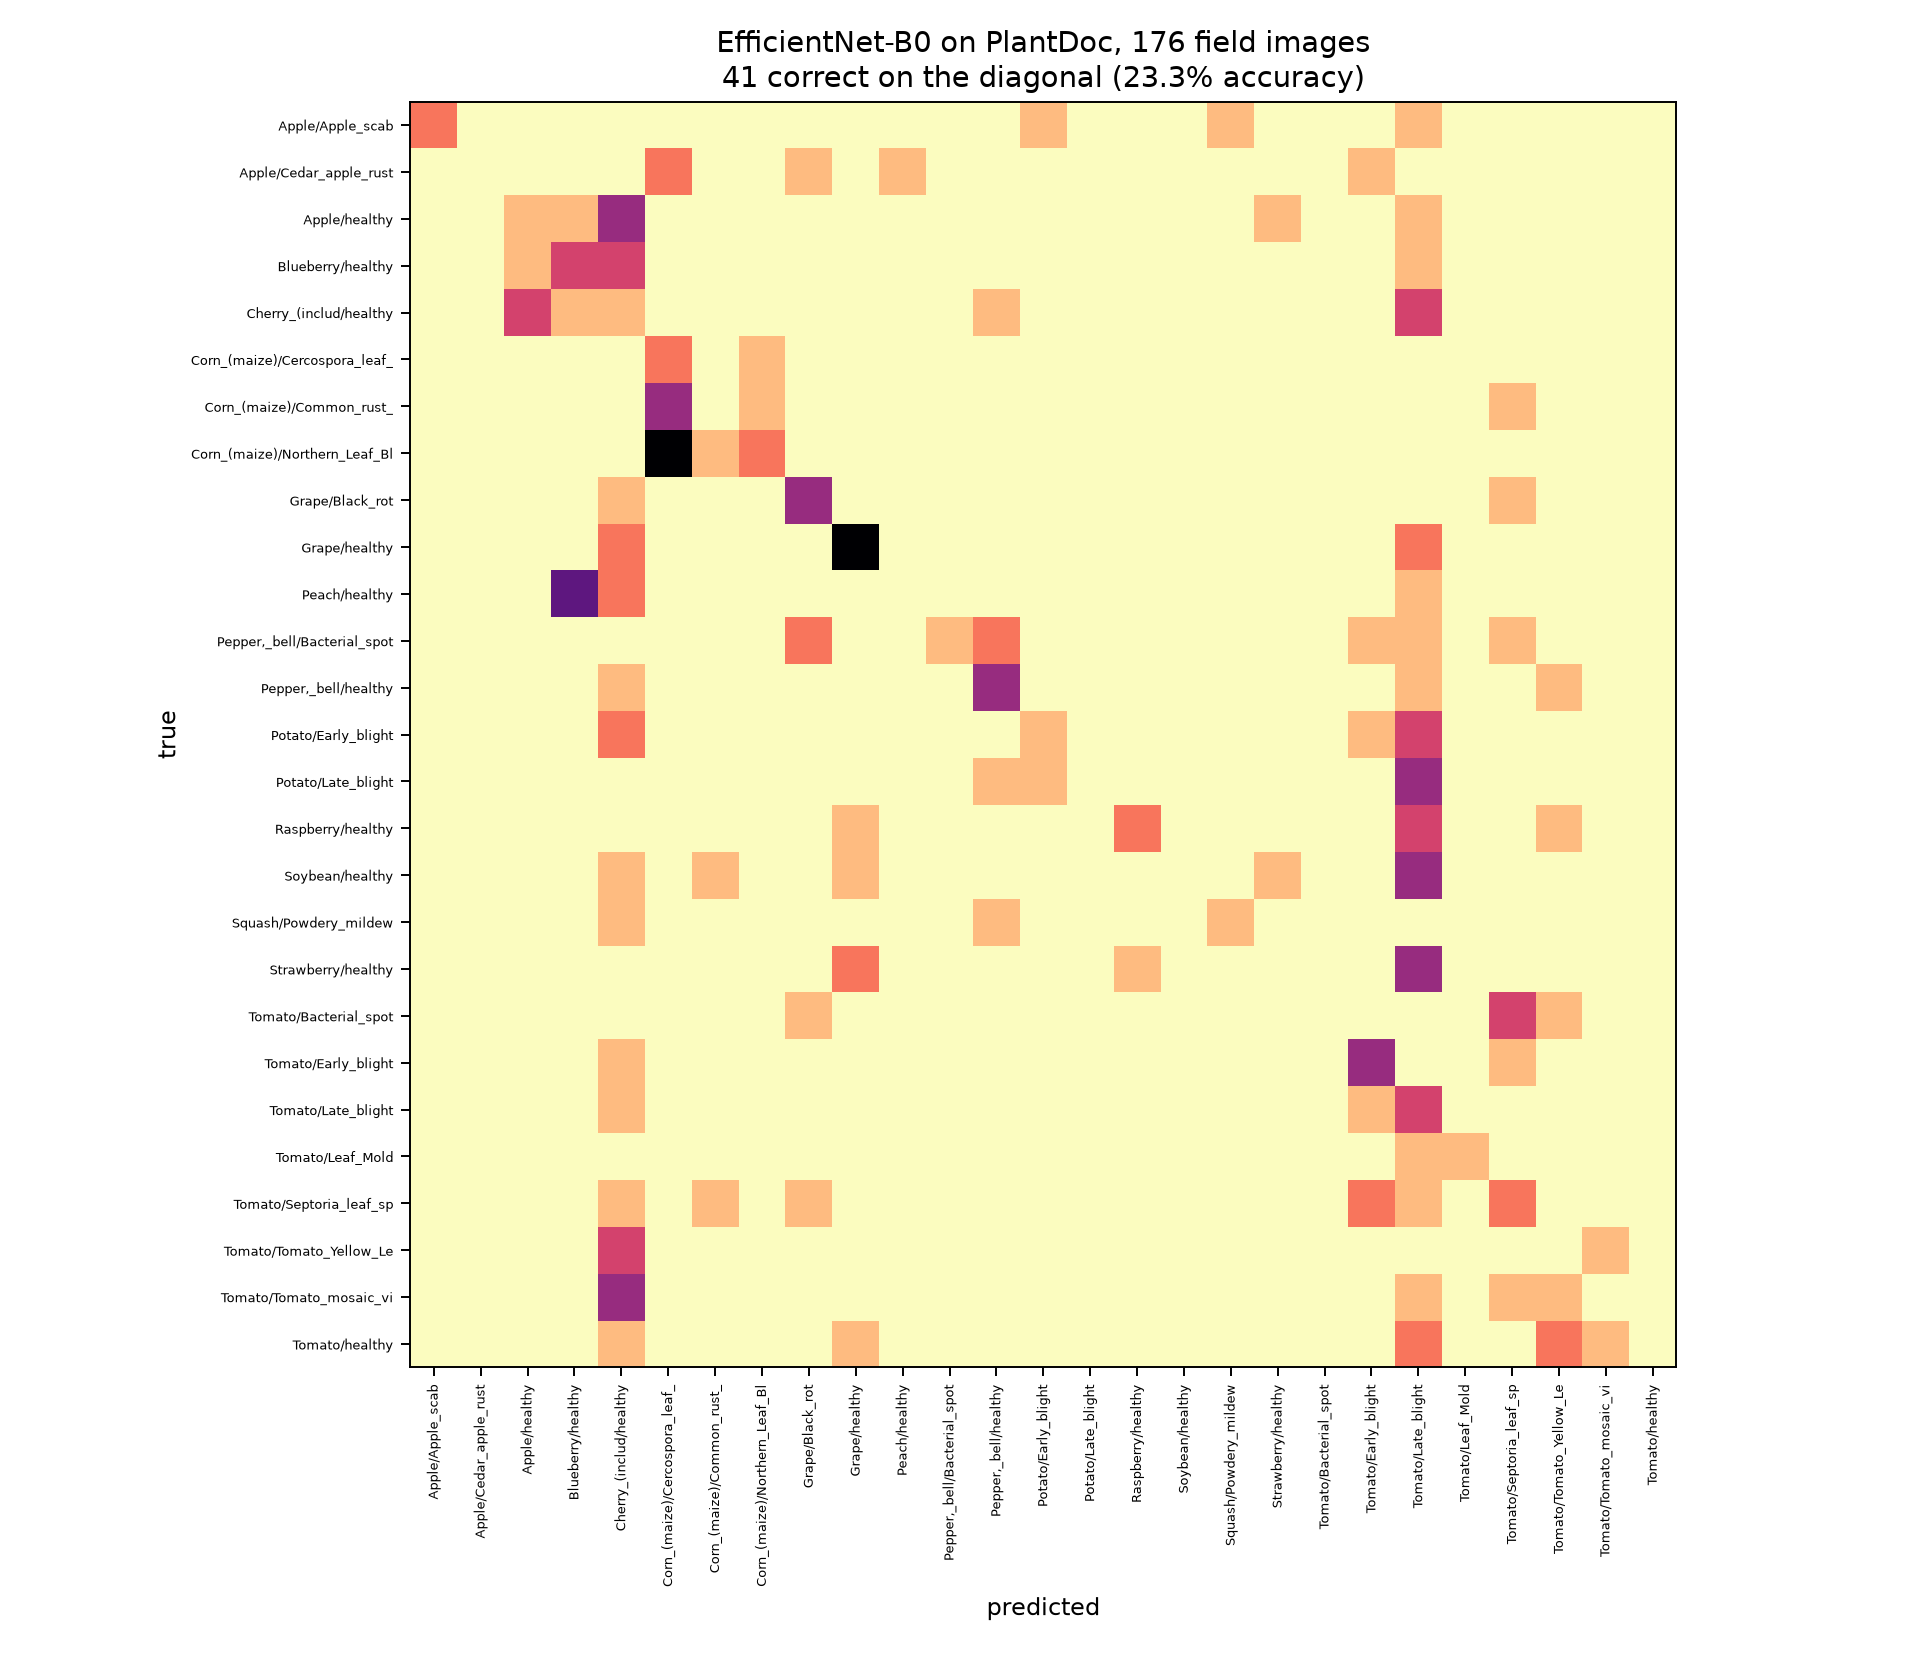
\includegraphics[width=0.78\textwidth]{fig_confusion.png}
\caption{Confusion structure on PlantDoc test. Off-diagonal mass is not confined to
neighbouring classes; predictions migrate to classes that PlantDoc does not contain,
which is the signature of a prior learned on a different label space.}
\label{fig:confusion}
\end{figure}

Field errors are not distributed evenly. Classes that depend on subtle lesion
morphology, such as rusts and blights, collapse to zero recall, while classes defined
by gross colour change survive better. The confusion structure shows predictions
migrating to visually similar classes and, in 21 to 29\,\% of cases, to a class
PlantDoc does not contain at all.

The second pattern is the more informative one. A model predicting a class outside
the field label space is not confusing two diseases; it is applying a prior learned
on a different problem. Confidence is high while this happens, which is why
abstention does not catch it.

\section{On explanation methods}

Grad-CAM produced plausible-looking maps that pointed at leaves. Taken alone, those
maps would have supported the wrong conclusion, since the model demonstrably uses
background as well. A heat map shows where the gradient is large, and a large
gradient is not the same as causal dependence.

\begin{figure}[H]
\centering
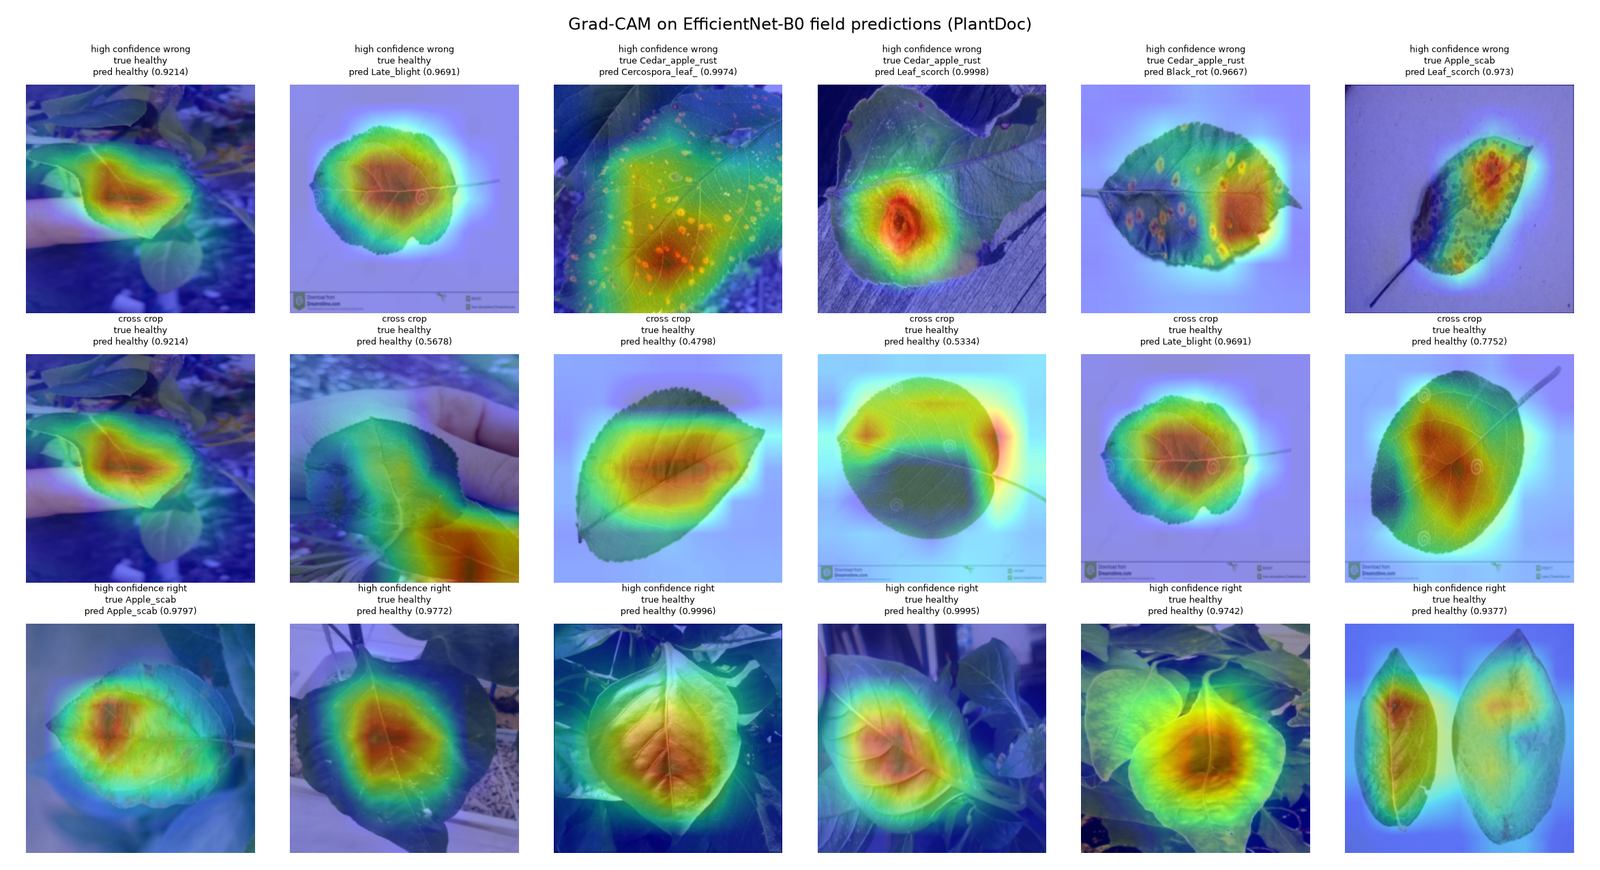
\includegraphics[width=0.95\textwidth]{fig_saliency.png}
\caption{Grad-CAM on four field cases, grouped by whether the prediction was correct
and how confident the model was. The maps look plausible and point at foliage. Taken
alone they would support the conclusion that the model reads the leaf, which the
intervention experiment later qualified.}
\label{fig:saliency}
\end{figure}

The intervention design cost one afternoon and produced an interpretable number with
an interval. For questions of the form ``what does this decision depend on'', it is
the better instrument, and its result contradicted the qualitative reading.

\section{What the system is worth}

On field images the reference model is correct about one time in five, is confident
when it is wrong, does not know which classes it cannot handle, and cannot be
repaired by thresholding. On curated images it is essentially perfect.

A system with that profile has no deployment case. What it has is diagnostic value:
it separates the part of the problem that is solved from the part that is not, and it
identifies leaf appearance under field conditions as the remaining problem.

\section{Implications for how this problem is reported}

Three reporting practices would have caught this earlier. Report the field number
beside the curated number, always, even when the field number is embarrassing.
Report an interval, because a 236-image estimate is not a point. And state what the
model depends on, measured rather than illustrated, because the plausible mechanism
and the true one turned out to be different.

None of these is expensive. All three change the conclusion.
